% Binary Tree Pointer Rotation
%
% File:         binary-tree-pointer-rotation.tex
% Author:       Bob Walton (walton@acm.org)
% Date:      	Thu Mar 28 19:19:21 EDT 2013
  
\documentclass{minimal}
\usepackage[paperheight=2.4in,paperwidth=6.2in,
            height=2.4in,hoffset=0.05in,
	    voffset=0.05in,left=0in,width=6.2in]{geometry}
\usepackage{color}
\usepackage[usenames]{xcolor}
\usepackage{tikz}
\usepackage{scalefnt}
\usetikzlibrary{arrows}
\begin{document}
\raggedright

\begin{tabular}{l}
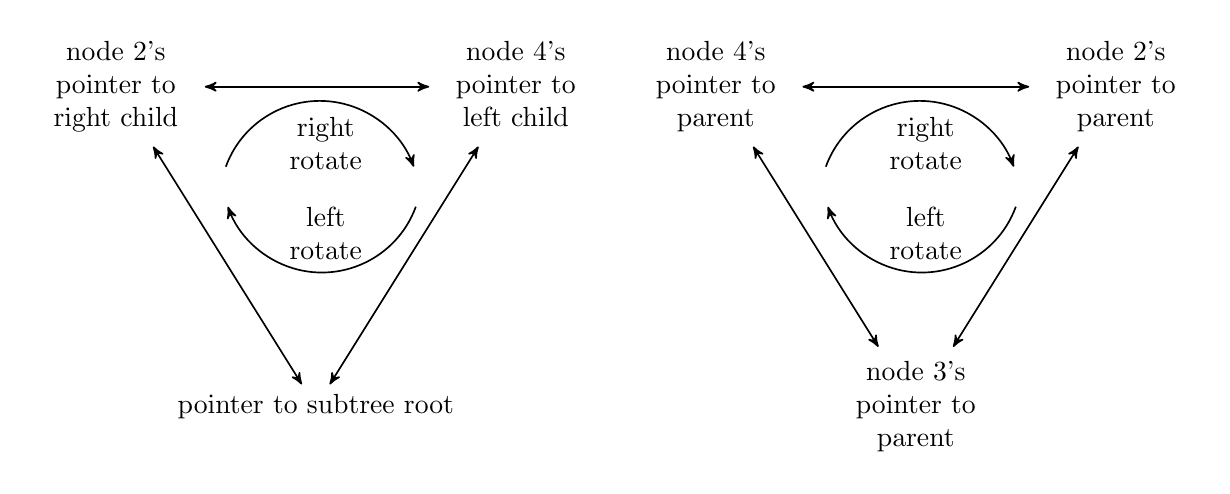
\begin{tikzpicture}[<->,>=stealth',auto,
                    semithick,
		    x=1in,y=1in]

\draw node (2R) at (1,1.8) {\begin{tabular}{c}node 2's\\
                                              pointer to\\
                                              right child\end{tabular}}
      node (4L) at (3,1.8) {\begin{tabular}{c}node 4's\\
                                              pointer to\\
                                              left child\end{tabular}}
      node (ROOT) at (2,0.2) {pointer to subtree root};

\path (2R) edge (4L)
      (4L) edge (ROOT)
      (ROOT) edge (2R);

\draw[->] (1.55,1.4) arc(160:20:0.5);
\node at(2.05,1.5) {\begin{tabular}{c}right\\rotate\end{tabular}};

\draw[->] (2.5,1.2) arc(-20:-160:0.5);
\node at(2.05,1.05) {\begin{tabular}{c}left\\rotate\end{tabular}};

\draw node (2P) at (4,1.8) {\begin{tabular}{c}node 4's\\
                                              pointer to\\
				   	      parent\end{tabular}}
      node (4P) at (6,1.8) {\begin{tabular}{c}node 2's\\
                                              pointer to\\
				   	      parent\end{tabular}}
      node (3P) at (5,0.2) {\begin{tabular}{c}node 3's\\
                                              pointer to\\
				   	      parent\end{tabular}};

\path (2P) edge (4P)
      (4P) edge (3P)
      (3P) edge (2P);

\draw[->] (4.55,1.4) arc(160:20:0.5);
\node at(5.05,1.5) {\begin{tabular}{c}right\\rotate\end{tabular}};

\draw[->] (5.5,1.2) arc(-20:-160:0.5);
\node at(5.05,1.05) {\begin{tabular}{c}left\\rotate\end{tabular}};

\end{tikzpicture}

\end{tabular}
\end{document}


